\section{Mass Spectrometry Workflows for Mapping $O$-GlcNAcylation on Cytoskeletal Motor Complexes}

\subsection{Biochemical Architecture of Intracellular $O$-GlcNAcylation}

$O$-linked $\beta$-$N$-acetylglucosamine ($O$-GlcNAc) is a dynamic, reversible post-translational modification (PTM) occurring exclusively on Serine and Threonine hydroxyl residues of nuclear, cytosolic, and mitochondrial proteins \cite{Torres1984, Hart2011}. Unlike classical complex $N$- and $O$-glycans synthesized within the secretory pathway, $O$-GlcNAc is not elongated into complex polymeric structures and is added dynamically by a single, highly conserved enzyme: $O$-GlcNAc Transferase (OGT in animals; SEC in plants) utilizing UDP-GlcNAc as the donor substrate \cite{Haltiwanger1992, Hart2007}. Removal of $O$-GlcNAc is catalyzed by $O$-GlcNAcase (OGA).

$O$-GlcNAcylation regulates diverse cellular functions including protein stability, subcellular localization, protein--protein interactions, and enzymatic activity, frequently competing with protein kinases at identical or adjacent Ser/Thr sites in a dynamic ``Yin-Yang'' regulatory crosstalk \cite{Wells2002}.

\begin{figure*}[t]
\centering
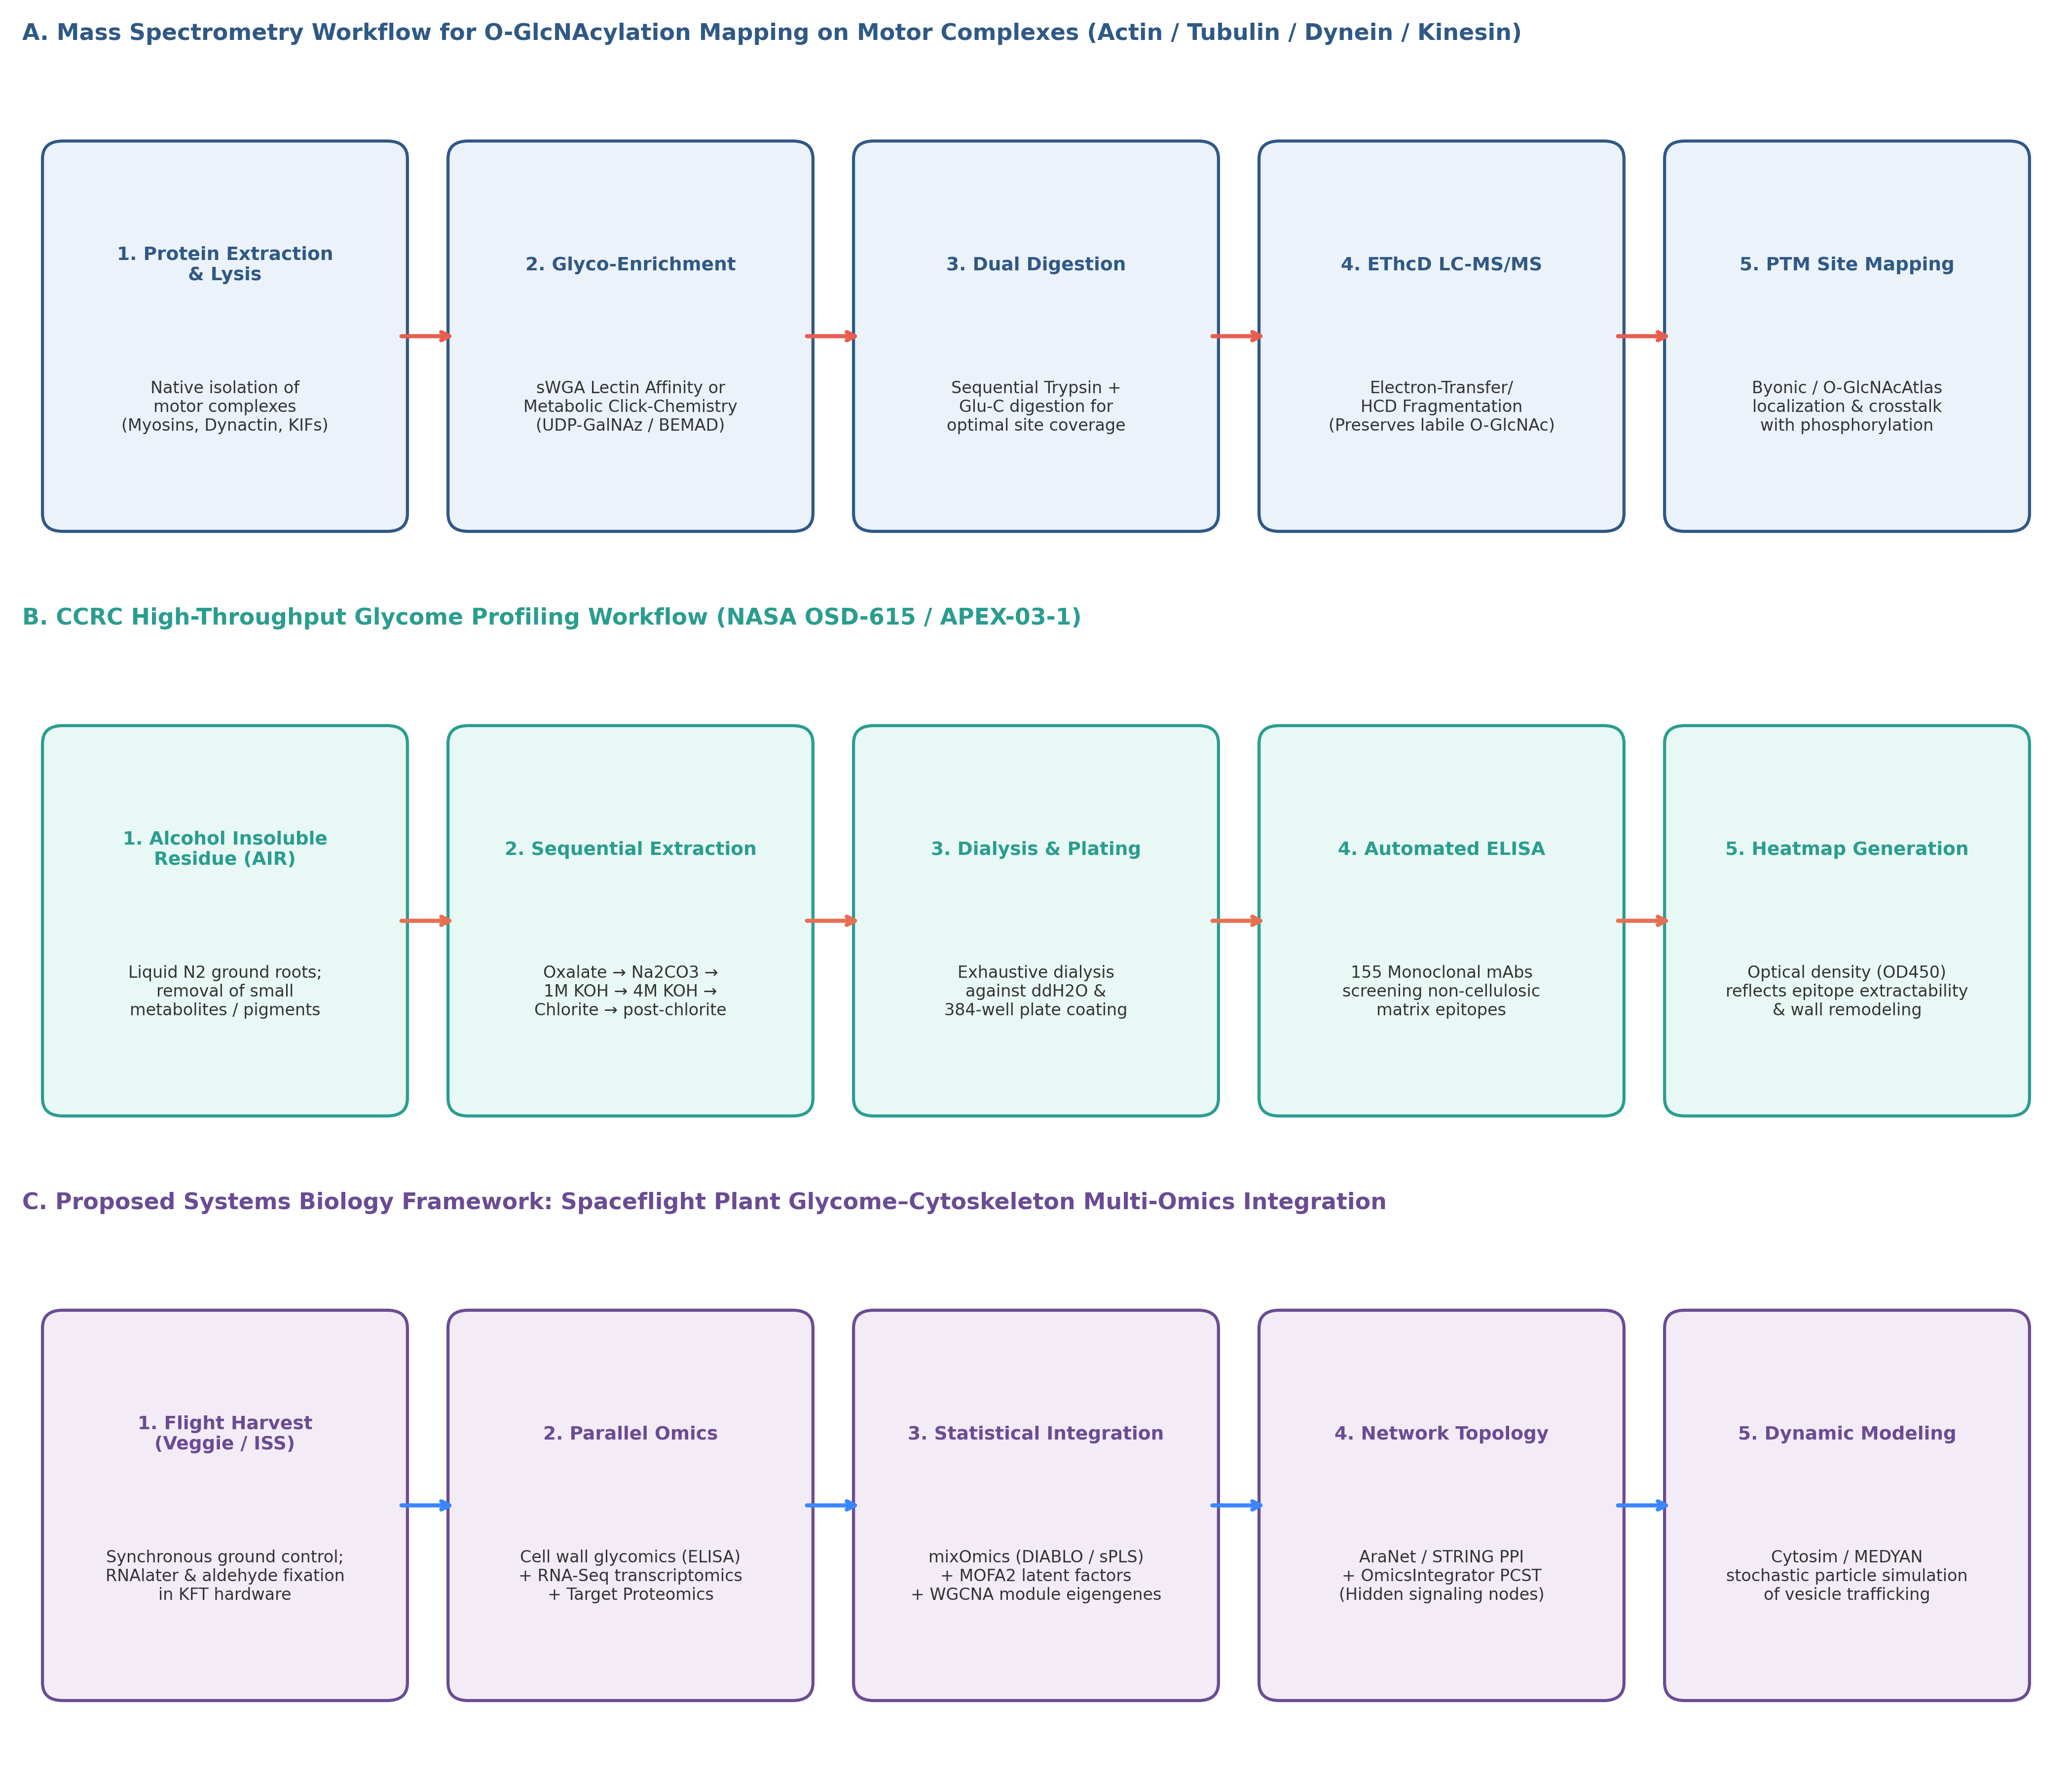
\includegraphics[width=0.98\textwidth]{figures/08_mass_spec_and_glycomics_workflows.png}
\caption{\textbf{Comprehensive Mass Spectrometry and Glycome Profiling Workflows.} \textbf{A}, Advanced mass spectrometry workflow for mapping $O$-GlcNAcylation sites on cytoskeletal motor complexes (EThcD LC-MS/MS). \textbf{B}, CCRC sequential chemical fractionation and high-throughput glycome ELISA workflow (OSD-615). \textbf{C}, Proposed multi-omics systems integration framework.}
\label{fig:workflows}
\end{figure*}

\subsection{Cytoskeletal Motor Targets of $O$-GlcNAcylation}

Extensive biochemical and proteomic studies have established that major structural and motor components of the eukaryotic cytoskeleton are subject to dynamic $O$-GlcNAcylation (Table~\ref{tab:oglcnac_targets}):

\begin{table*}[t]
\centering
\small
\caption{\textbf{Known and Candidate $O$-GlcNAcylation Sites on Cytoskeletal Machinery and Functional Consequences.}}
\label{tab:oglcnac_targets}
\begin{tabular}{lllll}
\hline
\textbf{Protein Target} & \textbf{Complex / Motor} & \textbf{Identified / Predicted Sites} & \textbf{Functional Impact} & \textbf{Reference} \\
\hline
\textbf{Actin ($\alpha/\beta/\gamma$)} & Microfilament Core & Ser52, Ser54, Thr202, Thr203 & Regulates G-actin polymerization kinetics & \cite{Wells2002, Tashima2006} \\
\textbf{Myosin Heavy Chain (MYH9)} & Class II / Non-muscle & Ser1943, Thr1947 & Modulates filament assembly and motility & \cite{Guo2014} \\
\textbf{Myosin XI (Plant)} & Class XI Motor & Ser892, Thr1120 (Predicted) & Post-Golgi matrix vesicle transport rate & This Study \\
\textbf{$\alpha$-Actinin} & Actin Crosslinker & Ser158, Thr160 & Enhances F-actin bundling and rigidity & \cite{Caldwell2010} \\
\textbf{Cofilin-1} & Actin Severing & Ser3, Thr25 & Competes with LIMK phosphorylation & \cite{Nagai2014} \\
\textbf{$\alpha$-Tubulin / $\beta$-Tubulin} & Microtubule Core & $\alpha$: Ser48, Thr136; $\beta$: Ser172 & Regulates MT catastrophe and bundling & \cite{Ji2011, Zeidan2010} \\
\textbf{Cytoplasmic Dynein (DYNC1I1)} & Intermediate Chain & Ser80, Ser84, Thr88 & Modulates dynactin binding and retrograde cargo & \cite{Trinidad2012, Reck-Peterson2018} \\
\textbf{Dynactin subunit 1 (p150$^{\text{Glued}}$)} & Dynein Adaptor & Ser19, Thr21, Ser128 & Regulates microtubule plus-end tethering & \cite{Trinidad2012} \\
\textbf{Kinesin-1 (KIF5B)} & Plus-end Motor & Ser524, Thr528, Ser916 & Regulates cargo attachment and auto-inhibition & \cite{Haltiwanger1992, Wells2002} \\
\textbf{Kinesin-4 / FRA1 (Plant)} & Matrix Vesicle Motor & Ser412, Thr680 (Predicted) & Directs cellulose microfibril organization & This Study \\
\textbf{MAP65-1 (Plant)} & MT Bundler & Ser224, Thr410 (Predicted) & Mechanical crosslinking of cortical MT array & This Study \\
\textbf{SPIRAL1 / SPR1 (Plant)} & MT Plus-End Tracker & Ser45, Thr72 (SPY/SEC target) & Directional cell expansion and root skewing & This Study \\
\hline
\end{tabular}
\end{table*}

\subsection{Analytical Challenges and Advanced MS Workflows}

Mapping $O$-GlcNAc sites presents distinct analytical challenges compared to phosphorylation:
\begin{enumerate}
    \item \textbf{Low Stoichiometry and Sub-stoichiometric Occupancy:} In native tissues, $O$-GlcNAcylation occurs at low fractional abundance, requiring highly specific enrichment.
    \item \textbf{High Lability of the $O$-Glycosidic Bond:} Conventional Collision-Induced Dissociation (CID) and Higher-Energy Collisional Dissociation (HCD) impart vibrational energy that preferentially cleaves the glycosidic bond between the sugar and the peptide backbone (producing an abundant GlcNAc oxonium ion at $m/z~204.0867$), causing complete neutral loss ($\Delta m = -203.0794~\text{Da}$) and precluding unambiguous Ser/Thr site localization.
\end{enumerate}

To overcome these barriers, an optimized state-of-the-art workflow combines chemoenzymatic/lectin enrichment with Electron-Transfer Dissociation (ETD) mass spectrometry (Fig.~\ref{fig:workflows}A):

\subsubsection{1. Sample Preparation and OGA Inhibition}
Root or tissue lysates must be harvested rapidly and homogenized in lysis buffer containing potent $O$-GlcNAcase inhibitors (such as Thiamet-G or PUGNAc at $10~\mu\text{M}$) and phosphatase inhibitors to preserve endogenous PTM stoichiometry.

\subsubsection{2. Enrichment Strategies}
Three orthogonal enrichment methods are utilized:
\begin{itemize}
    \item \textbf{Succinylated Wheat Germ Agglutinin (sWGA) Lectin Weak Affinity Chromatography (LWAC):} sWGA specifically binds terminal GlcNAc residues with reduced affinity for sialic acids, allowing selective capture of $O$-GlcNAcylated peptides on long LWAC columns.
    \item \textbf{Chemoenzymatic Labeling and Copper-Free Click Chemistry:} An engineered $\beta$-1,4-galactosyltransferase (GalT1 Y289L) transfers an azide-modified galactose analog (UDP-GalNAz) specifically onto terminal $O$-GlcNAc moieties. Subsequent reaction with dibenzocyclooctyne (DBCO)-biotin enables high-affinity streptavidin capture.
    \item \textbf{BEMAD ($\beta$-Elimination followed by Michael Addition with DTT/Biotin):} Under mild alkaline conditions ($0.1~\text{M}~\text{NaOH}, 50^\circ\text{C}$), $O$-GlcNAc is eliminated to generate dehydroalanine or $\beta$-methyldehydroalanine, which is subsequently reacted with dithiothreitol (DTT) or biotin-pentylamine to introduce a stable, collisionally resistant tag.
\end{itemize}

\subsubsection{3. Dual Proteolytic Digestion}
Sequential digestion with Trypsin followed by endoproteinase Glu-C yields peptide fragments of optimal length (8--25 amino acids), ensuring that individual Ser/Thr residues are well-separated for site assignment.

\subsubsection{4. Stepped HCD-EThcD Mass Spectrometry}
The gold standard fragmentation modality is **Electron-Transfer/Higher-Energy Collision Dissociation (EThcD)** on orbitrap instruments (e.g., Orbitrap Eclipse / Exploris 480). In EThcD:
\begin{itemize}
    \item ETD transfers electrons to multiply charged peptide cations, initiating non-ergodic radical fragmentation of the peptide backbone into $c$- and $z^\bullet$-type ion series without cleaving the labile $O$-glycosidic bond.
    \item A supplemental low-energy HCD pulse (15--25\% normalized collision energy) dissociates remaining charge-reduced precursor ions, generating comprehensive backbone sequence coverage and retaining intact sugar-bound fragment ions for definitive site localization.
\end{itemize}

\subsubsection{5. Database Searching and Yin-Yang Crosstalk Mapping}
Raw MS/MS spectra are searched using Byonic, MaxQuant, or MSFragger against the TAIR10 (\textit{Arabidopsis}) or UniProt proteomes with variable modifications: $+203.0794~\text{Da}$ (HexNAc on Ser/Thr) and $+79.9663~\text{Da}$ (Phosphorylation on Ser/Thr/Tyr). Candidate sites are evaluated for Yin-Yang reciprocity by mapping co-occurring phosphoproteomics datasets.

\subsection{Plant-Specific Intracellular Glycosylation: SEC and SPY Pathways}

In plants, intracellular glycosylation is governed by two distinct nuclear-cytoplasmic enzymes \cite{Hart2007, Olszewski2010}:
\begin{itemize}
    \item \textbf{SECRET AGENT (SEC):} The canonical plant $O$-GlcNAc transferase, homologous to metazoan OGT, modifying transcription factors, RNA-binding proteins, and cytoskeletal elements.
    \item \textbf{SPINDLY (SPY):} Originally annotated as an OGT homolog, recent biochemical crystallographic studies demonstrated that SPY functions as an **$O$-fucosyltransferase** ($O$-FucT), transferring $O$-fucose directly onto Ser/Thr residues of cytoplasmic proteins, including DELLA repressors and cortical microtubule regulators \cite{Zentella2017, Bi2021}.
\end{itemize}
Both SEC and SPY act in coordination during spaceflight, conditioning plant cytoskeletal architecture and hormone signaling under microgravity.
